\documentclass[12pt]{article}

\usepackage{sbc-template}
\usepackage{graphicx,url}
\usepackage[T1]{fontenc}
\usepackage[utf8]{inputenc}
\usepackage[brazilian]{babel}
\usepackage{xurl}
\usepackage{booktabs}
\usepackage[section]{placeins}

\graphicspath{{../figuras/}}

\sloppy

\title{Gravidade dos acidentes nas rodovias federais brasileiras}

\author{Felipe da Silva Araújo\inst{1}, Fernando Gabriel Feitosa Leite\inst{1},\\
  Karllisson Henrique da Silva\inst{1}}

\address{Instituto de Computação -- Universidade Federal de Alagoas (UFAL)\\
  Maceió -- AL -- Brasil}

\begin{document}

\maketitle

\begin{abstract}
  Using the Federal Highway Police (PRF) records of 506,404 crashes with victims on Brazilian federal highways from 2017 to 2025, we study which factors and places are associated with fatal outcomes. Hypothesis tests show that the odds of a crash being fatal are 2.3 times higher at night than during the day and 2.2 times higher on single-carriageway roads, while head-on collisions and pedestrian crashes account for 13\% of the crashes and 46\% of the fatal ones. A LightGBM classifier evaluated on 2024--2025 reaches a PR-AUC of 0.36, against 0.085 for the base rate. Refitted on the crash profile alone, it estimates the expected number of fatal crashes in each 10~km segment; the segments most above expectation in 2017--2022 remained 1.6 times above it in 2024--2025. We propose priorities for enforcement and road improvements, with success criteria based on comparable segments.
\end{abstract}

\begin{resumo}
  A partir dos registros da Polícia Rodoviária Federal (PRF) de 506.404 acidentes com vítimas nas rodovias federais de 2017 a 2025, estudamos quais fatores e locais estão associados aos acidentes fatais. Testes de hipótese mostram que a chance de um acidente ser fatal é 2,3 vezes maior à noite do que de dia e 2,2 vezes maior em pista simples, e que colisões frontais e atropelamentos de pedestres somam 13\% dos acidentes e 46\% dos fatais. Um classificador LightGBM avaliado em 2024--2025 atinge PR-AUC de 0,36, contra 0,085 da taxa base. Reajustado só com o perfil dos acidentes, ele estima quantos acidentes fatais seriam esperados em cada trecho de 10~km; os trechos mais acima do esperado em 2017--2022 seguiram com 1,6 vez o esperado em 2024--2025. Propomos prioridades de fiscalização e de melhoria das vias, com critérios de sucesso baseados em trechos comparáveis.
\end{resumo}

\section{Aplicação}

De 2017 a 2025, a Polícia Rodoviária Federal (PRF) registrou mais de 50 mil mortes nas rodovias federais, mais de 5 mil a cada ano. Nem todo acidente, porém, tem a mesma consequência: uma colisão pode deixar apenas feridos em um trecho e mortos em outro. Como a PRF registra cada ocorrência com as condições do acidente e o seu desfecho, é possível ir além da contagem de casos e perguntar o que diferencia os acidentes fatais dos demais.

Este trabalho procura responder a essa pergunta e mostrar onde e quando esses acidentes se concentram, no país e em Alagoas. Como exercício de apoio à decisão, simulamos a escolha de onde e quando concentrar a fiscalização e a prevenção nas rodovias, com operações, controle de velocidade, campanhas e pedidos de melhoria da via. A base da PRF atende aos critérios do projeto final da disciplina de Ciência de Dados do IC/UFAL~\cite{disciplina}: é grande, mistura variáveis numéricas e categóricas, tem um desfecho claro e exige preparação antes da modelagem. Na análise, combinamos testes de hipótese, modelos de classificação e um ranking de trechos que compara os acidentes fatais observados com os esperados pelo perfil dos acidentes de cada trecho.

\section{Base de dados}

Os dados vêm do conjunto ``Acidentes -- agrupados por ocorrência'' dos Dados Abertos da PRF~\cite{prf}, publicado em arquivos anuais. De 2017, quando a PRF passou a usar o sistema de registro BAT~\cite{prfdicionario}, a 2025, último ano completo, são 632.713 ocorrências e 30 colunas, iguais em todos os anos. Cada registro traz as seguintes informações:
\begin{itemize}
  \item \textbf{tempo:} data, dia da semana, horário e fase do dia;
  \item \textbf{local:} UF, município, BR, km, coordenadas e unidade da PRF;
  \item \textbf{via e contexto:} tipo de pista, traçado, uso do solo, sentido, condição meteorológica, causa e tipo do acidente;
  \item \textbf{envolvidos:} pessoas e veículos, com o número de mortos, feridos, ilesos e ignorados;
  \item \textbf{resultado:} classificação do acidente como sem vítimas, com vítimas feridas ou com vítimas fatais.
\end{itemize}

Na série mensal por classe (Figura~\ref{fig:classes}), os acidentes sem vítimas caem para menos da metade a partir de abril de 2018, enquanto os acidentes com feridos e com mortos seguem estáveis. Uma mudança tão brusca, só nessa classe, indica uma alteração na forma de registro. Por isso, analisamos apenas os acidentes com vítimas, e o alvo passa a ser se o acidente foi fatal ou não. Nesse recorte, a proporção de fatais fica entre 8,2\% e 8,8\% em todos os anos.

\begin{figure}[ht]
\centering
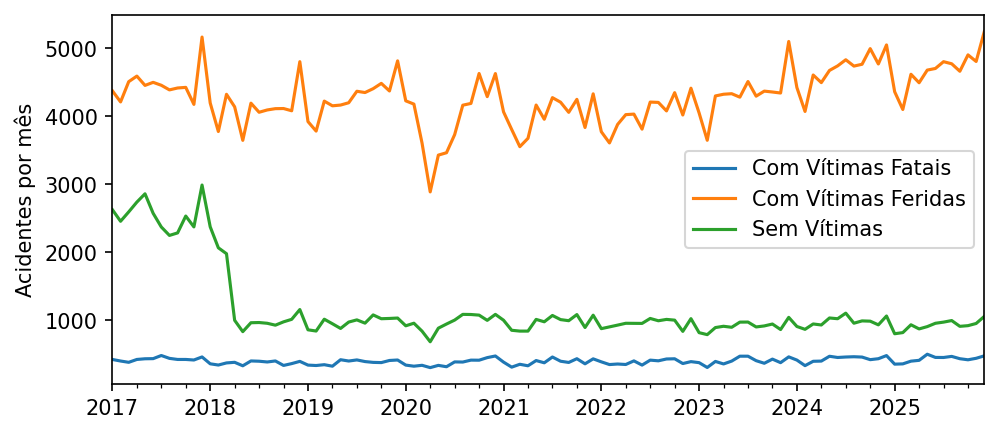
\includegraphics[width=\textwidth]{acidentes_por_classe.png}
\caption{Acidentes por mês em cada classe. Os acidentes sem vítimas mudam de patamar em abril de 2018.}
\label{fig:classes}
\end{figure}

\subsection{Pré-processamento}

A preparação e as análises foram feitas em Python, com pandas~\cite{pandas} e NumPy~\cite{numpy}, em um notebook Jupyter entregue com este artigo; as figuras foram feitas com matplotlib~\cite{matplotlib} e seaborn~\cite{seaborn}. Dez ocorrências repetiam outra em tudo menos no identificador e foram removidas. Dez classificações vazias foram recuperadas pelas contagens de vítimas, com a regra que reproduz todas as classificações preenchidas (fatal se há mortos, com feridos se há feridos e sem vítimas nos demais casos). Coordenadas fora do Brasil (54) e o número de BR igual a zero (1.407, as mesmas ocorrências com sentido ``Não Informado'') foram tratados como ausentes. Em 872 ocorrências (0,17\%), a fase do dia é incompatível com a hora, como pleno dia de madrugada; elas foram mantidas. As categorias ``Ignorado'' e ``Não Informado'' de clima e sentido foram mantidas como categorias próprias.

As categorias também mudam ao longo do tempo. Os 21 tipos de acidente foram reduzidos a 15, porque colisão lateral e colisão com objeto mudam de subdivisão em 2020--2021, e os 41 registros sem tipo ficaram em ``Outros''. As 91 descrições de causa mudam de nomenclatura quase inteira em 2021, e as agrupamos por palavras-chave em 11 grupos: pedestre, álcool e drogas, velocidade, sono e saúde, desatenção e reação, manobra ou infração, veículo, animais, clima, via e outros. Mesmo assim, a divisão entre desatenção e manobra ainda muda em 2021. O traçado da via pode ter vários valores na mesma ocorrência e virou 12 variáveis binárias. Criamos também a hora, a faixa horária, o mês, o ano, o fim de semana e o feriado nacional, este a partir da biblioteca holidays~\cite{holidays}; Carnaval e Corpus Christi não são feriados nacionais e ficaram de fora.

Depois dessas etapas, restam 506.404 acidentes com vítimas, dos quais 43.438 (8,6\%) são fatais. Como a classificação é definida pelas contagens de mortos e feridos, essas contagens, assim como as de ilesos e ignorados, não foram usadas como preditoras. O número de pessoas e o de veículos envolvidos foram mantidos.

\section{Estatística descritiva e inferência}

Os acidentes com vítimas envolvem em média 2,64 pessoas e 1,98 veículos, com desvios padrão de 2,11 e 1,08, mediana de 2 nos dois casos e máximos de 95 e 131, uma distribuição bastante assimétrica. A Figura~\ref{fig:variaveis} mostra a taxa de fatais por categoria das principais variáveis. Em plena noite, 12,5\% dos acidentes com vítimas são fatais, e ao amanhecer, 13,3\%, contra 5,9\% em pleno dia. Em pista simples a taxa é de 11,5\%, o dobro da pista dupla (5,8\%). Colisões frontais (30,7\%) e atropelamentos de pedestres (28,7\%) se destacam de todos os outros tipos, e a causa ligada a pedestres tem a maior taxa entre os grupos de causa. Já a chuva (7,7\%) fica abaixo do céu claro (8,9\%).

\begin{figure}[ht]
\centering
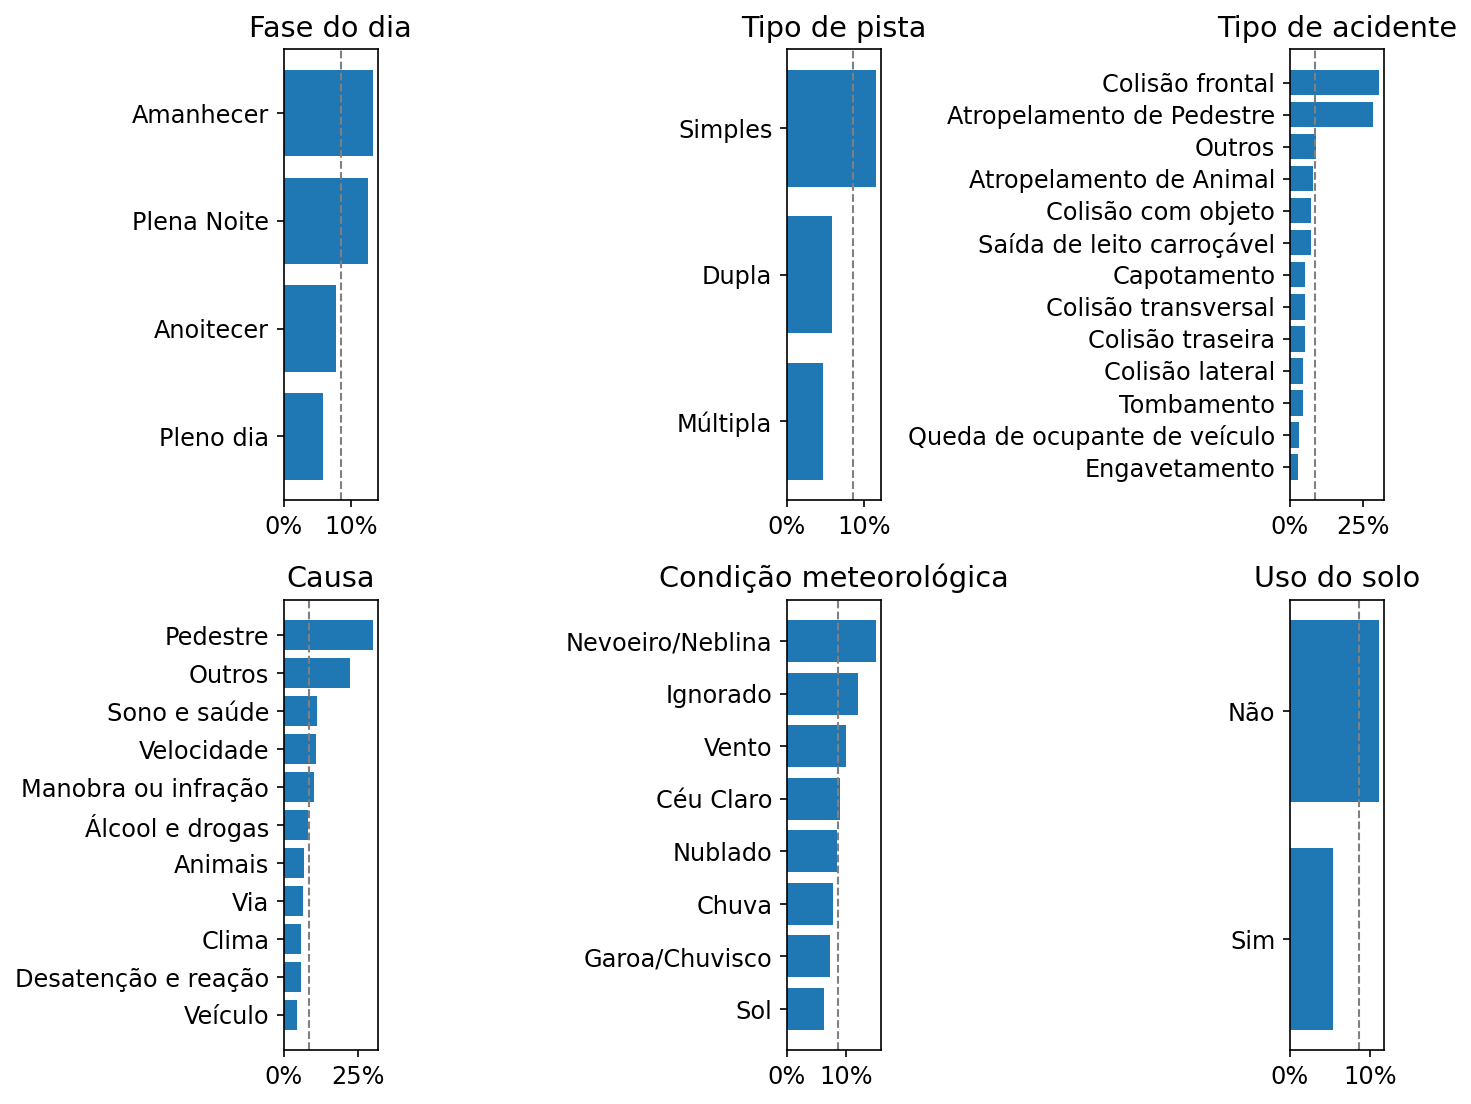
\includegraphics[width=\textwidth]{taxa_por_variavel.png}
\caption{Taxa de fatais entre os acidentes com vítimas, por categoria. A linha tracejada é a taxa nacional (8,6\%); categorias com menos de 500 acidentes foram omitidas.}
\label{fig:variaveis}
\end{figure}

Pelo V de Cramér~\cite{scipyassociacao}, calculado a partir da estatística qui-quadrado~\cite{scipy}, o tipo do acidente é a variável mais associada ao desfecho (0,30), seguido da causa (0,18); fase do dia e faixa horária se sobrepõem bastante (0,56), assim como tipo e causa (0,42). No tempo, a letalidade se concentra nas madrugadas e noites, sobretudo nos fins de semana (Figura~\ref{fig:diahora}), e as madrugadas e noites de sábado e domingo reúnem 15,4\% dos acidentes e 24,6\% dos fatais.

\begin{figure}[ht]
\centering
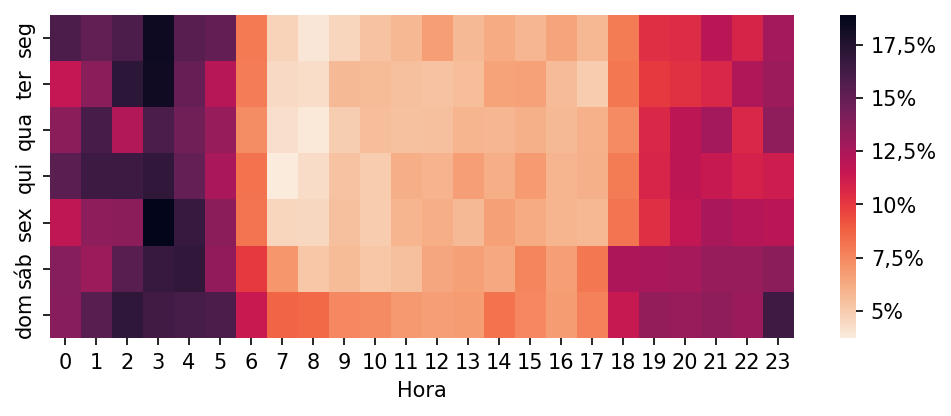
\includegraphics[width=\textwidth]{taxa_dia_hora.png}
\caption{Taxa de fatais por dia da semana e hora.}
\label{fig:diahora}
\end{figure}

No espaço, os acidentes são mais letais no Norte e no Nordeste (Figura~\ref{fig:mapa}). Maranhão (21,3\%) e Pará (18,3\%) têm as maiores taxas, contra 5,0\% em Santa Catarina e no Distrito Federal. Alagoas, com 4.643 acidentes com vítimas, tem taxa de 14,6\%, acima da nacional em todas as fases do dia; a chance de um acidente ser fatal no estado é 1,84 vez a das demais UFs (IC 95\%: 1,69--1,99).

\begin{figure}[ht]
\centering
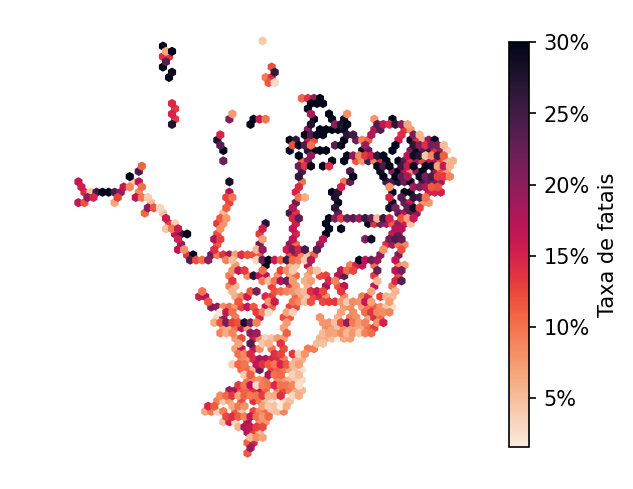
\includegraphics[width=.6\textwidth]{mapa_taxa.png}
\caption{Taxa de fatais por região, em hexágonos com pelo menos 30 acidentes; a escala de cor para em 30\%.}
\label{fig:mapa}
\end{figure}

As hipóteses da proposta foram testadas com o teste qui-quadrado e com a razão de chances e seu intervalo de 95\%, calculados com SciPy~\cite{scipy} e statsmodels~\cite{statsmodels}:
\begin{enumerate}
  \item[\textbf{H1.}] Em plena noite, a proporção de acidentes fatais é maior do que em pleno dia.
  \item[\textbf{H2.}] Em pista simples, a proporção de acidentes fatais é maior do que em pistas duplas ou múltiplas.
  \item[\textbf{H3.}] Colisões frontais e atropelamentos de pedestres concentram uma parcela desproporcional dos acidentes fatais.
  \item[\textbf{H4.}] Em fins de semana e feriados, a proporção de acidentes fatais é maior do que em dias úteis.
  \item[\textbf{H5.}] A proporção de acidentes fatais sob chuva não é maior do que com céu claro ou sol.
\end{enumerate}
Com centenas de milhares de acidentes, quase toda diferença é estatisticamente significativa, então o que importa é o tamanho do efeito. O nível de significância foi corrigido por Bonferroni para os cinco testes ($\alpha = 0{,}01$). Pela Tabela~\ref{tab:hipoteses}, todas as diferenças são significativas, e as cinco hipóteses se confirmam. Em H3, os dois tipos somam 13,1\% dos acidentes e 45,7\% dos fatais. Em H5, a taxa sob chuva é menor que com céu claro ou sol; uma explicação possível é que se dirige mais devagar na chuva, mas a base não permite verificar isso.

\begin{table}[ht]
\centering
\caption{Taxa de fatais nos grupos comparados e razão de chances (RC) com intervalo de 95\%. Em todos os testes, $p < 0{,}001$.}
\label{tab:hipoteses}
\small
\begin{tabular}{llrlrr}
\toprule
 & Grupo A & Taxa & Grupo B & Taxa & RC (IC 95\%) \\
\midrule
H1 & plena noite & 12,5\% & pleno dia & 5,9\% & 2,29 (2,24--2,34) \\
H2 & pista simples & 11,5\% & dupla ou múltipla & 5,6\% & 2,19 (2,15--2,24) \\
H3 & frontal ou pedestre & 29,8\% & demais tipos & 5,4\% & 7,50 (7,34--7,66) \\
H4 & fim de semana ou feriado & 10,2\% & dia útil & 7,7\% & 1,36 (1,34--1,39) \\
H5 & chuva & 7,7\% & céu claro ou sol & 8,7\% & 0,89 (0,86--0,92) \\
\bottomrule
\end{tabular}
\end{table}

\section{Métodos avaliados}

Para estimar a chance de um acidente com vítimas ser fatal, foram comparados três classificadores, implementados com scikit-learn~\cite{sklearnlogistica} e LightGBM~\cite{lightgbm}. O primeiro é uma referência que atribui a todo acidente a taxa de fatais do treino. O segundo é uma regressão logística, cujos coeficientes se leem como razões de chances. Nela, cada variável categórica usa como referência a categoria mais frequente no treino, o mês entra como categoria, com janeiro como referência, categorias com menos de 100 acidentes no treino são agrupadas, as contagens de pessoas e veículos entram em escala logarítmica e padronizadas, para conter os valores extremos, e o ajuste é feito sem penalização. O terceiro é o LightGBM, um modelo de \textit{gradient boosting} com árvores de decisão que trata variáveis categóricas diretamente e capta relações não lineares e interações; usamos taxa de aprendizado de 0,05, até 63 folhas por árvore, pelo menos 100 acidentes por folha e 80\% das linhas e das colunas sorteadas a cada árvore, e o número de árvores (134) foi definido por parada antecipada na validação, depois de 100 árvores sem melhora da PR-AUC.

As preditoras são UF, BR, fase do dia, faixa horária, dia da semana, condição meteorológica, tipo de pista, uso do solo, tipo e causa do acidente, feriado, as 12 variáveis de traçado, mês e os números de pessoas e de veículos. Deixamos de fora o sentido da via. O valor ``Não Informado'' coincide exatamente com a BR ausente, o que impede estimar a regressão logística com as duas variáveis, e tiramos o sentido também do LightGBM. Já a faixa horária fica só no LightGBM: ela se sobrepõe à fase do dia, e na regressão logística o efeito da noite se dividiria entre as duas. Para interpretar o LightGBM, foram usados os valores SHAP calculados pelo próprio LightGBM~\cite{lightgbm} em uma amostra de 20 mil acidentes do teste.

Para a priorização de trechos, o LightGBM foi reajustado só com o perfil de cada acidente (tipo, causa, fase do dia, faixa horária, dia da semana, clima, feriado, mês e números de pessoas e de veículos), sem o local nem as características da via. Com validação cruzada em cinco partes consecutivas, de cerca de dois anos cada~\cite{sklearncv}, cada acidente recebe uma probabilidade estimada por um modelo que não o viu no ajuste. A soma dessas probabilidades em cada trecho de 10~km de uma BR em uma UF é o número de fatais esperado para o perfil dos acidentes do trecho, e a diferença entre observados e esperados é o excesso. Como tipo de pista, traçado e uso do solo ficam fora do perfil, o excesso também inclui o efeito deles.

\section{Métricas de avaliação}

Com apenas 8,6\% de fatais, a acurácia diz pouco, já que prever sempre ``não fatal'' acerta 91,5\% dos acidentes do teste. A métrica principal é a área sob a curva de precisão e revocação (PR-AUC), uma medida útil quando as classes são muito desbalanceadas~\cite{sklearnpr}; a área sob a curva ROC (ROC-AUC) é reportada como complemento. Para ilustrar o compromisso entre acertos e alarmes, também são apresentadas a precisão, a revocação e a matriz de confusão em um limiar de decisão. Como o ranking de trechos soma probabilidades, também foi verificada a calibração, isto é, se as probabilidades previstas correspondem às frequências observadas.

\section{Método de avaliação}

A divisão entre treino, validação e teste segue a ordem do tempo. O treino usa 2017--2022 (326.791 acidentes), a validação, 2023 (56.803), e o teste, 2024--2025 (122.810). Essa divisão simula o uso do modelo em anos que ele ainda não viu e expõe o efeito das mudanças de registro ao longo do tempo, que uma divisão aleatória esconderia. Usamos a validação para a parada antecipada do LightGBM e para escolher o limiar que maximiza o F1 (0,22), e o teste foi usado uma única vez, no fim, para avaliar os classificadores. A proporção de fatais é semelhante nos três conjuntos (8,6\%, 8,6\% e 8,5\%). Não foram usados pesos de classe, para manter as probabilidades calibradas; o desbalanceamento é tratado pela métrica e pela escolha do limiar.

\section{Resultados e discussão}

\subsection{Desempenho dos modelos}

A Tabela~\ref{tab:modelos} mostra o desempenho na validação e no teste. O LightGBM tem o melhor resultado, com PR-AUC de 0,363 no teste, cerca de quatro vezes a da referência, e a regressão logística fica pouco atrás; a vantagem do LightGBM, de 0,030, tem intervalo bootstrap de 95\% de 0,026 a 0,034 e aparece em 2024 e em 2025. Os valores praticamente não mudam da validação para o teste, o que indica que os modelos se mantêm nos anos mais recentes. No limiar escolhido, o LightGBM encontra 47\% dos acidentes fatais do teste, e 37\% dos acidentes que ele aponta como fatais de fato o são. As probabilidades previstas pelo LightGBM são bem calibradas no teste.

\begin{table}[ht]
\centering
\caption{Desempenho dos modelos na validação (2023) e no teste (2024--2025).}
\label{tab:modelos}
\begin{tabular}{lrrrr}
\toprule
 & \multicolumn{2}{c}{Validação} & \multicolumn{2}{c}{Teste} \\
Modelo & PR-AUC & ROC-AUC & PR-AUC & ROC-AUC \\
\midrule
Referência & 0,086 & 0,500 & 0,085 & 0,500 \\
Regressão logística & 0,338 & 0,812 & 0,333 & 0,814 \\
LightGBM & 0,365 & 0,830 & 0,363 & 0,834 \\
\bottomrule
\end{tabular}
\end{table}

Tipo e causa só são conhecidos depois do acidente, então o modelo não serve para antecipar acidentes. Ele foi usado para medir o peso de cada fator com os demais controlados e para estimar quantos fatais seriam esperados em cada trecho.

\subsection{Fatores associados à morte}

Nos dois modelos, o tipo do acidente é o fator mais forte. Na regressão logística, atropelamento de pedestre e colisão frontal multiplicam a chance de morte por 6,2 e 5,1 em relação à colisão traseira. Mesmo descontando as demais variáveis, plena noite e amanhecer quase dobram a chance em relação ao pleno dia (razões de 1,97 e 2,04, com intervalos de 1,91--2,03 e 1,93--2,16), e as pistas dupla e múltipla a reduzem em 20\% e 23\% em relação à simples. No LightGBM (Figura~\ref{fig:shap}), depois do tipo vêm o número de veículos, o uso do solo, a UF e a fase do dia, com pouca diferença entre esses quatro; entre as causas, velocidade, sono ou saúde do condutor e as ligadas a pedestres são as que mais aumentam a chance de morte. Esses resultados confirmam, com os demais fatores controlados, o que as hipóteses H1 a H3 indicavam.

\begin{figure}[ht]
\centering
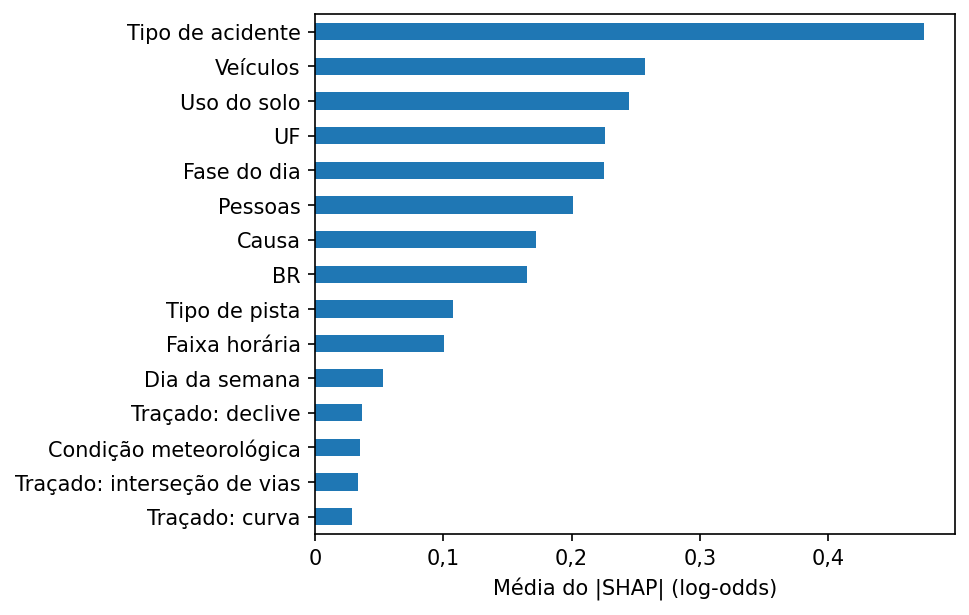
\includegraphics[width=.75\textwidth]{shap.png}
\caption{Importância das variáveis no LightGBM: média do valor SHAP absoluto, em log-odds.}
\label{fig:shap}
\end{figure}

\FloatBarrier
\subsection{Onde e quando priorizar}

Entre os 6.757 trechos de 10~km com acidentes, os 107 com pelo menos 34 fatais reúnem 11,9\% dos acidentes fatais. Essa concentração persiste no tempo, mas reflete em boa parte o movimento das vias. Os 107 trechos com pelo menos 23 fatais em 2017--2022 tiveram 11\% dos fatais de 2024--2025, mas também 20\% dos acidentes com vítimas; em geral, são trechos movimentados, com taxa de fatais abaixo da média.

\begin{table}[ht]
\centering
\caption{Trechos com maior excesso de acidentes fatais sobre o esperado pelo perfil dos acidentes, 2017--2025.}
\label{tab:excesso}
\begin{tabular}{lrrrr}
\toprule
Trecho & Acidentes & Fatais & Esperados & Obs./esp. \\
\midrule
MA, BR-316, km 610--620 & 157 & 52 & 21,9 & 2,4 \\
PE, BR-232, km 50--60 & 206 & 44 & 18,6 & 2,4 \\
PA, BR-316, km 20--30 & 251 & 44 & 21,6 & 2,0 \\
PE, BR-232, km 210--220 & 82 & 35 & 12,6 & 2,8 \\
AL, BR-101, km 170--180 & 108 & 33 & 15,9 & 2,1 \\
\bottomrule
\end{tabular}
\end{table}

O ranking pelo excesso sobre o esperado favorece bem menos os trechos movimentados. Os 50 trechos com maior excesso têm mediana de 97 acidentes, contra mais de mil entre os 50 com mais fatais. O modelo de perfil é bem calibrado, com 43.458 fatais esperados para 43.438 observados e razão entre observados e esperados de 0,97 a 1,05 em cada ano. A Tabela~\ref{tab:excesso} mostra os cinco trechos com maior excesso, e a Figura~\ref{fig:mapatrechos}, onde ficam os 40 primeiros, em sua maioria no Nordeste e no Pará, em parte porque a letalidade desses estados é mais alta para o mesmo perfil de acidente. Os 50 trechos com maior excesso em 2017--2022 tinham 2,2 vezes os fatais esperados nesse período e, em 2024--2025, tiveram 265 fatais para 163 esperados (1,6 vez). Com o esperado ajustado pela letalidade de cada UF em 2017--2022, que vai de 0,65 vez o esperado em Santa Catarina a 1,88 no Maranhão, o ranking muda, e os 50 primeiros passaram de 1,8 para 1,3 vez o esperado (303 fatais para 235 esperados). Como esses trechos foram escolhidos justamente por estarem acima do esperado, parte do excesso some por regressão à média. No ranking nacional, cerca de metade dele se manteve e, com o ajuste por UF, pouco mais de um terço; o que resta aponta para efeitos da região e dos próprios trechos. Com o modelo de perfil ajustado só com 2017--2022, o resultado é o mesmo (1,6 vez, com 48 dos 50 trechos em comum).

\begin{figure}[ht]
\centering
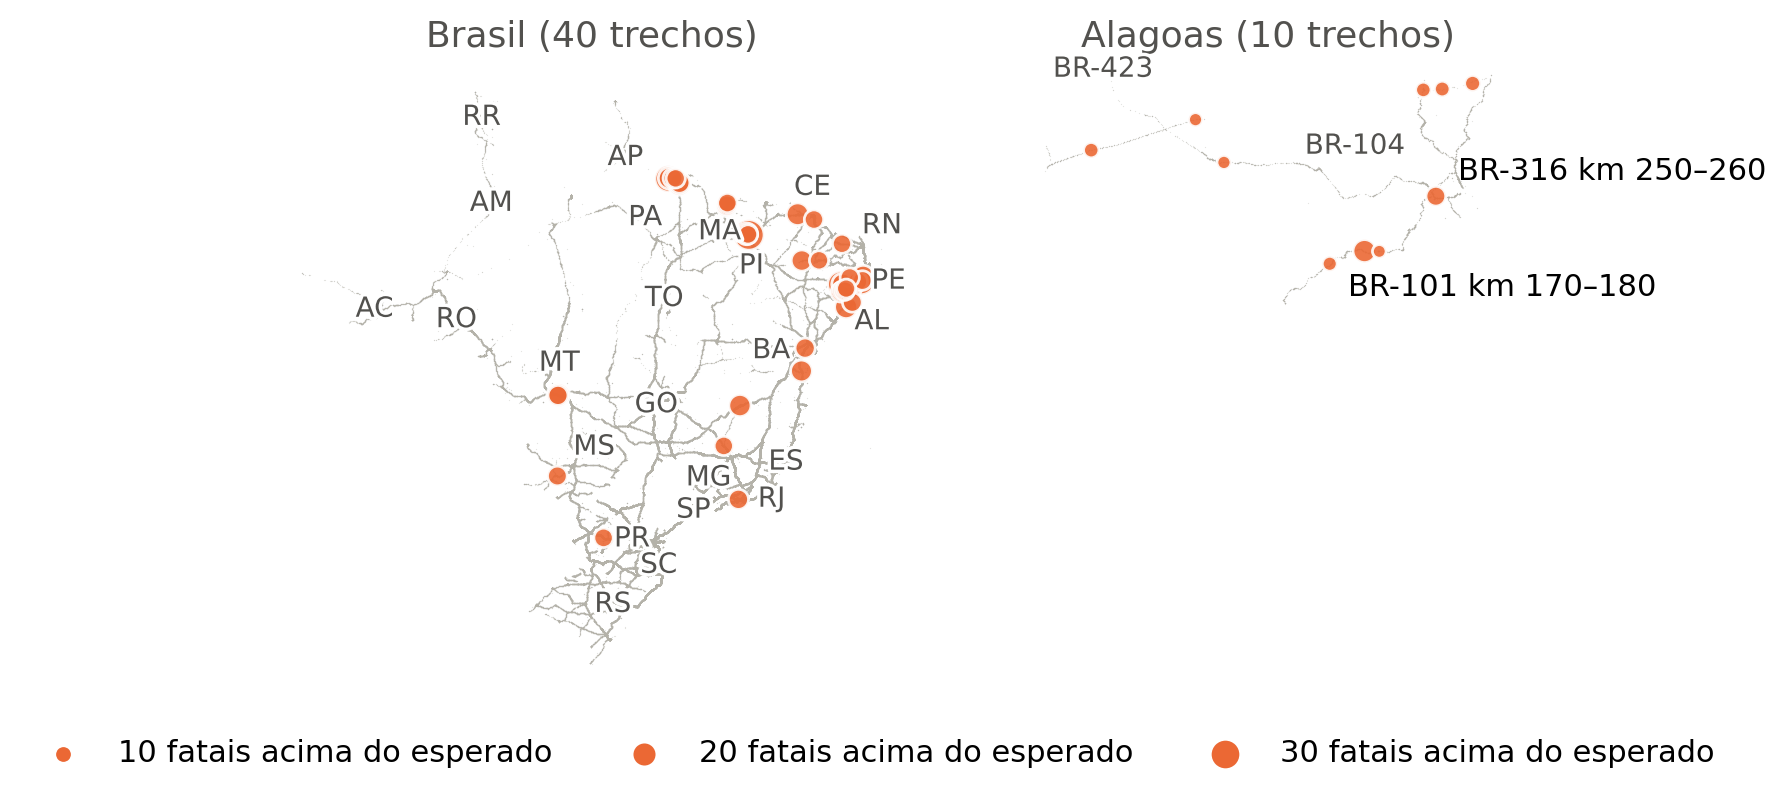
\includegraphics[width=\textwidth]{mapa_trechos.png}
\caption{Trechos com maior excesso de acidentes fatais sobre o esperado, no Brasil e em Alagoas. A área do círculo é proporcional ao excesso; o fundo cinza são os locais dos acidentes, que desenham as rodovias.}
\label{fig:mapatrechos}
\end{figure}

Em Alagoas (Figura~\ref{fig:mapatrechos}, à direita), o trecho do km 170 ao 180 da BR-101 lidera o excesso, com 33 fatais em 108 acidentes com vítimas, o dobro do esperado; segue-se o do km 250 ao 260 da BR-316, com 31 fatais para 18,4 esperados.

\FloatBarrier
\subsection{Recomendações}

\textbf{Noite em pista simples.} Em pista simples, 15,6\% dos acidentes com vítimas em plena noite são fatais, e 17,1\% ao amanhecer; de dia, em pista dupla ou múltipla, são 3,4\%. As madrugadas e noites de sábado e domingo concentram 25\% dos fatais com só 15\% dos acidentes. Além de H1, H2 e H4, a regressão logística mostra que o efeito da noite e da pista simples se mantém mesmo descontando as demais variáveis, o que aponta para vias sem separação de sentidos durante a noite. Recomendamos reforçar a fiscalização e a sinalização noturna nos trechos de pista simples com mais acidentes fatais à noite, começando pelas noites de fim de semana. Em 12 meses, a taxa de fatais à noite nos trechos escolhidos deveria cair pelo menos 10\% em relação a trechos não priorizados com histórico semelhante, com o número de acidentes com vítimas como acompanhamento.

\textbf{Colisões frontais e atropelamentos.} Esses dois tipos somam 13\% dos acidentes com vítimas, mas 46\% dos fatais (H3), e são os que mais pesam nos dois modelos. Desde 2021, quase dois terços das colisões frontais têm como causa uma manobra ou infração, sobretudo contramão e ultrapassagem indevida, e um terço delas é fatal. Propomos fiscalizar ultrapassagens e pedir faixas adicionais ou separação central nos trechos onde as colisões frontais se repetem, e iluminação e travessias seguras onde há atropelamentos. O indicador é o número de colisões frontais e atropelamentos fatais nesses trechos, acompanhado pelo total de acidentes com vítimas. Como trechos escolhidos por terem muitos casos tendem a melhorar um pouco por conta própria, a meta é uma queda de pelo menos 10\% em 12 meses em relação a trechos não priorizados com histórico semelhante.

\textbf{Lista anual de trechos.} O número de fatais e o excesso sobre o esperado apontam trechos diferentes, e os dois se mantiveram de 2017--2022 para 2024--2025. Por isso, sugerimos uma lista anual de trechos prioritários com as duas medidas. O número de fatais orienta a fiscalização, e o excesso, a inspeção e os pedidos de melhoria da via onde se morre mais do que o perfil dos acidentes explica. No ano seguinte, a participação desses trechos nos acidentes fatais deveria cair mais do que em trechos de histórico semelhante fora da lista, e a razão entre fatais observados e esperados serve de acompanhamento.

\textbf{Alagoas.} Em Alagoas, a chance de um acidente com vítimas ser fatal é 1,84 vez a das demais UFs, e a taxa é mais alta em todas as fases do dia, então o horário dos acidentes não explica a diferença. Os trechos do estado com maior excesso, a começar pelo km 170--180 da BR-101, deveriam encabeçar o planejamento local da fiscalização e dos pedidos de melhoria da via. Em 12 meses, a razão entre fatais observados e esperados nesses trechos deveria cair mais do que em trechos de Alagoas com histórico semelhante que ficaram fora da lista, com o número de acidentes fatais no estado como acompanhamento.

Pela H5, operações motivadas só pela chuva não são prioridade.

\subsection{Limitações}
\label{sec:limitacoes}

Os resultados valem para acidentes com vítimas: os sem vítimas ficaram de fora pela quebra de registro de 2018. As taxas são calculadas por acidente, já que a base não traz o fluxo de veículos; um trecho com muitos fatais pode ser só um trecho movimentado. Tipo e causa só são conhecidos depois do acidente, então o modelo explica a gravidade, mas não antecipa acidentes. O agrupamento das causas não elimina toda a mudança de nomenclatura de 2021, e outros campos também mudam de registro ao longo dos anos, como o traçado em 2023 e a troca gradual de capotamento por tombamento. Em cerca de 5\% das ocorrências o número de pessoas é menor que a soma das contagens de vítimas, o que acontece mais nos acidentes fatais e afeta essa variável preditora; sem ela, a PR-AUC do LightGBM na validação vai de 0,365 a 0,361, e 48 dos 50 trechos do ranking se repetem. O excesso sobre o esperado depende das variáveis de perfil disponíveis, e parte dele pode vir de fatores do acidente que a base não registra, como a velocidade no impacto ou o uso de cinto e capacete. Por fim, as associações encontradas não provam causa.

\section{Conclusão}

Este trabalho analisou 506.404 acidentes com vítimas nas rodovias federais de 2017 a 2025 para entender o que torna um acidente fatal e onde isso acontece mais. A preparação dos dados tratou duplicatas, classificações ausentes, coordenadas inválidas, mudanças de nomenclatura e uma quebra de registro que levou ao recorte nos acidentes com vítimas. Os testes de hipótese e os modelos apontam na mesma direção. Colisões frontais e atropelamentos, a noite e a madrugada e a pista simples estão entre os fatores mais associados à morte, e Norte e Nordeste concentram os acidentes mais letais, com Alagoas bem acima da média nacional. O LightGBM teve o melhor desempenho e, reajustado com o perfil dos acidentes, permitiu identificar trechos que matam mais do que o esperado de forma persistente. As principais limitações, discutidas na Seção~\ref{sec:limitacoes}, são a falta de dados de fluxo de veículos e o fato de o modelo explicar a gravidade sem antecipar acidentes.

Como trabalhos futuros, dados de fluxo de veículos permitiriam medir o risco por quilômetro percorrido, e um painel interativo permitiria consultar o ranking de trechos por estado e por ano.

\bibliographystyle{sbc}
\bibliography{referencias}

\end{document}
